\documentclass[a4paper,12pt]{article} % тип документа

% Поля страниц
\usepackage[left=2.5cm,right=2.5cm,
    top=2cm,bottom=2cm,bindingoffset=0cm]{geometry}
    
%Пакет дял таблиц   
\usepackage{multirow} 
    
%Отступ после заголовка    
\usepackage{indentfirst}


% Рисунки
\usepackage{floatrow,graphicx,calc}
\usepackage{wrapfig}

%%% Работа с картинками
\usepackage{graphicx}  % Для вставки рисунков
\graphicspath{{images/}{images2/}}  % папки с картинками
\setlength\fboxsep{3pt} % Отступ рамки \fbox{} от рисунка
\setlength\fboxrule{1pt} % Толщина линий рамки \fbox{}
\usepackage{wrapfig} % Обтекание рисунков и таблиц текстом

% Создаёем новый разделитель
\DeclareFloatSeparators{mysep}{\hspace{1cm}}

% Ссылки?
\usepackage{hyperref}
\usepackage[rgb]{xcolor}
\hypersetup{				% Гиперссылки
    colorlinks=true,       	% false: ссылки в рамках
	urlcolor=blue          % на URL
}


%  Русский язык
\usepackage[T2A]{fontenc}			% кодировка
\usepackage[utf8]{inputenc}			% кодировка исходного текста
\usepackage[english,russian]{babel}	% локализация и переносы




% Математика
\usepackage{amsmath,amsfonts,amssymb,amsthm,mathtools}

%%% Дополнительная работа с математикой
\usepackage{amsmath,amsfonts,amssymb,amsthm,mathtools} % AMS
\usepackage{icomma} % "Умная" запятая: $0,2$ --- число, $0, 2$ --- перечисление


% Что-то 
\usepackage{wasysym}


\begin{document}
\begin{center}
	\footnotesize{ФЕДЕРАЛЬНОЕ ГОСУДАРСТВЕННОЕ АВТОНОМНОЕ ОБРАЗОВАТЕЛЬНОЕ 			УЧРЕЖДЕНИЕ ВЫСШЕГО ОБРАЗОВАНИЯ}\\
	\footnotesize{МОСКОВСКИЙ ФИЗИКО-ТЕХНИЧЕСКИЙ ИНСТИТУТ\\(НАЦИОНАЛЬНЫЙ 			ИССЛЕДОВАТЕЛЬСКИЙ УНИВЕРСИТЕТ)}\\
	\footnotesize{ФАКУЛЬТЕТ ОБЩЕЙ И ПРИКЛАДНОЙ ФИЗИКИ\\}
	\hfill \break
	\hfill \break
	\hfill \break
	\hfill \break
\end{center}


\begin{figure*}[h]
    \centering
    \includegraphics*[width=10cm,height=7cm,keepaspectratio]{mipt_eng_text_png.png}
    \label{fig:my_label}
\end{figure*}


\begin{center}   
    \hfill \break
	\hfill \break
	\hfill \break
	\large{Лабораторная работа № 4.1.2\\ \hfill \break\Large{Моделирование оптических приборов и определение их увеличения}}\\
	\hfill \break
	\hfill \break
	\hfill \break
	\begin{flushright}
		Баранов Даниил\\
		Группа Б02-103
	\end{flushright}
	\hfill \break
	\hfill \break
	\hfill \break
\end{center}
\hfill \break
\hfill \break
\hfill \break
\hfill \break
\begin{center}
	Долгопрудный, 2023 г.
\end{center}
\thispagestyle{empty}

\newpage

\textbf{Используются в работе:}  оптическая скамья, набор линз, экран, осветитель со шкалой, зрительная труба, диафрагма, линейка.

\textbf{Экспериментальная установка.} Набор линз, осветитель, экран, зрительная труба, необходимые для моделирования оптических приборов, устанавливаются при помощи рейтеров на оптической скамье. Предметом служит миллиметровая шкала или сетка, нанесённая на матовое стекло осветителя.

\textbf{Центрирование линз.} При юстировке любых оптических приборов важно правильно центрировать входящие в систему линзы. Проходя через плохо отцентрированную систему линз, лучи света отклоняются в сторону и могут вообще не доходить до глаза наблюдателя. Центрировать линзы следует как по высоте, так и в поперечном направлении (для чего линзы крепятся на поперечных салазках). Подробно с правилами центрировки Вы познакомитесь при выполнении задания.

\textbf{Юстировка коллиматора.} При составлении моделей телескопических систем необходимо иметь удалённый объект. В качестве такого объекта обычно используется бесконечно удалённое изображение предмета (шкалы осветителя), установленного в фокальной плоскости положительной линзы. Лучи, выходящие из одной точки предмета, пройдя через линзу, образуют параллельный пучок. Устройство такого рода называется коллиматором.

Для юстировки коллиматора удобно использовать вспомогательную зрительную трубу, предварительно настроенную на бесконечность. Передвигая линзу коллиматора вдоль скамьи, добиваются появления резкого изображения предмета в окуляре зрительной трубы.

\textbf{Измерение фокусных расстояний линз.} Для того, чтобы сознательно моделировать оптические инструменты, нужно знать фокусные расстояния линз, которые могут быть использованы в качестве объектива или окуляра модели. Фокусные расстояния тонких положительных линз проще всего найти с помощью вспомогательной зрительной трубы, установленной на бесконечность. Работа выполняется так же, как при юстировке коллиматора.

При определении фокусного расстояния отрицательной линзы предметом служит изображение шкалы, которое даёт вспомогательная положительная линза.

\section{Ход работы}
\subsection{Определение фокусных расстояний тонких линз с помощью зрительной трубы}
\begin{enumerate}
    \item Из имеющегося набора линз отберём собирающие и рассеивающие: с помощью собирающих удаётся получить изображение удалённого объекта, с помощью рассеивающих нет. Получилось 4 собирающих и 1 рассеивающая.
    \item Соберём и отцентрируем установку.
    \item Настроим зрительную трубу на бесконечность: наведём трубу на удалённый объект и настроим на резкое видение окулярной шкалы.
    \item  Поставим собирающую линзу на расстоянии от предмета, примерно равном фокусному. На небольшом расстоянии от линзы закрепим трубу, настроенную на бесконечность, и отцентрируем её по высоте. Диафрагма диаметром d = 1 см, надетая на ближнюю к осветителю линзу, уменьшит сферические аберрации и повысит чёткость изображения. При этом расстояние между предметом и серединой тонкой линзы (между проточками на оправах) равно её фокусному расстоянию. Пункту соответствует \textbf{рисунок 1}.
    \item Для определения фокусного расстояния тонкой рассеивающей линзы сначала получим на экране увеличенное изображение сетки при помощи одной короткофокусной собирающей линзы. Измерим расстояние $a_{0} = 30 \pm 0,1$ см между линзой и экраном. Разместите сразу за экраном трубу, настроенную на бесконечность, и
закрепите её. Уберём экран и поставим на его место исследуемую рассеивающую линзу. Перемещая рассеивающую линзу, найдём в окуляре зрительной трубы резкое изображение сетки. Измерив расстояние между линзами ℓ, рассчитайте фокусное расстояние рассеивающей линзы $f = l - a_{0}$. Пункту соответствует \textbf{рисунок 2}.

\item Результаты измерений пунктов 4 и 5 представлены в \textbf{таблице 1}.
	\begin{figure}[h]
 \centering
 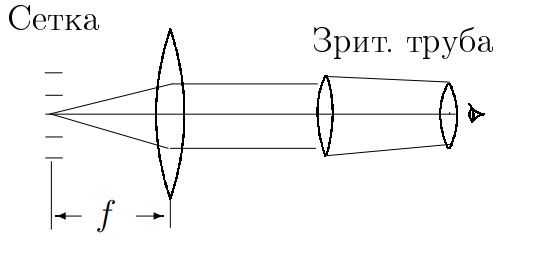
\includegraphics[scale=0.8]{lab_pic1.jpg}
		\caption{Определение фокусного расстояния собирающей линзы}
		
	\end{figure}
 	\begin{figure}[h]
 \centering
 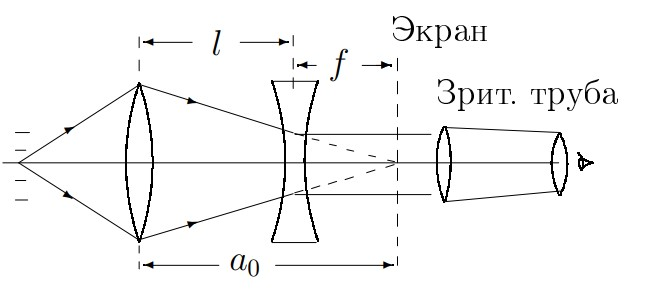
\includegraphics[scale=0.8]{lab_pic2.jpg}
		\caption{Определение фокусного расстояния рассеивающей линзы}
		
	\end{figure}
\end{enumerate}
\begin{table}[h]
\centering
\begin{tabular}{|llll|}

\hline
\multicolumn{4}{|l|}{Фокусные расстояние}                                                                                 \\ \hline
\multicolumn{2}{|l|}{Собирающие линзы}                                  & \multicolumn{2}{l|}{Рассеивающие линзы}         \\ \hline
\multicolumn{1}{|l|}{$f_{1}$, см} & \multicolumn{1}{l|}{$8,0 \pm 0,5$}  & \multicolumn{1}{l|}{$f_{5}$, см} & $-8,0 \pm 0,5$ \\ \hline
\multicolumn{1}{|l|}{$f_{2}$, см} & \multicolumn{1}{l|}{$10,0 \pm 0,5$} & \multicolumn{1}{l|}{}            &              \\ \hline
\multicolumn{1}{|l|}{$f_{3}$, см} & \multicolumn{1}{l|}{$18,7 \pm 0,5$} & \multicolumn{1}{l|}{}            &              \\ \hline
\multicolumn{1}{|l|}{$f_{4}$, см} & \multicolumn{1}{l|}{$28,1 \pm 0,5$} & \multicolumn{1}{l|}{}            &              \\ \hline
\end{tabular}
\caption{Результаты измерения фокусных расстояний линз}
\end{table}
\newpage
\subsection{Телескоп Кеплера}
\begin{enumerate}
    \item Из имеющегося набора отберём две собирающие линзы с фокусными расстояниями $f_{1} = 28,1 \pm 0,5$ см и $f_{2} = 8,0 \pm 0,5$ см. В качестве коллиматора используем линзы с фокусным расстоянием $18,7 \pm 0,5$ см. Настроим коллиматор с помощью зрительной трубы и наденем на него диафрагму.
    \item Определим размер изображения $h_{1} = 9 \pm 0,5$ одного миллиметра шкалы осветителя в делениях окулярной шкалы зрительной трубы.
    \item Соберём модель телескопа: линзу с максимальным фокусным расстоянием — объектив телескопа — расположим почти вплотную к линзе коллиматора, окуляр — на расстоянии, примерно равном сумме фокусных расстояний обеих линз трубы. Пункту соответствует \textbf{рисунок 3}.
    \item Слегка
перемещая окуляр телескопа вдоль оптической скамьи, получим изображение сетки в объективе вспомогательной трубы.
Измерим расстояние между объективом и окуляром телескопа и
сравним его с суммой фокусных расстояний. Получилось $s = 36,5$ см, что в пределах погрешности совпадает с суммой фокусных расстояний.
\item Рассчитаем увеличение исследуемой модели телескопа по формуле
\begin{equation}
    N_{\text{Т}} = -\frac{f_{1}}{f_{2}} = -3,5 \pm 0,2
\end{equation}
\item Найдём размер $h_{2} = 33 \pm 0,5$ изображения миллиметрового деления шкалы осветителя в делениях окулярной шкалы при наблюдении \textbf{по схеме рисунка 3}. Рассчитаем искомое увеличение по формуле
\begin{equation}
        N_{\text{Т}} = -\frac{h_{2}}{h_{1}} = -3,7 \pm 0,2
\end{equation}
\item Измерим диаметр $D_{1} = 34 \pm 1$ мм оправы объектива и диаметр $D_{2} = 9 \pm 1$  изображения этой оправы в окуляре. Для этого отодвинем вспомогательную трубу и расположим экран за окуляром телескопа. Снимем диафрагму с коллиматора. Отодвигая экран от окуляра, получим чёткое изображение оправы объектива.
\item Рассчитаем увеличение по формуле 
\begin{equation}
        N_{\text{Т}} = -\frac{D_{1}}{D_{2}} = 3,8 \pm 0,4
\end{equation}
\item Погрешность результата - увеличения телескопа - в этом пункте получилась довольно большой, однако три способа расчёта сошлись в пределах погрешности.
\end{enumerate}

 \begin{figure}[h]
 \centering
 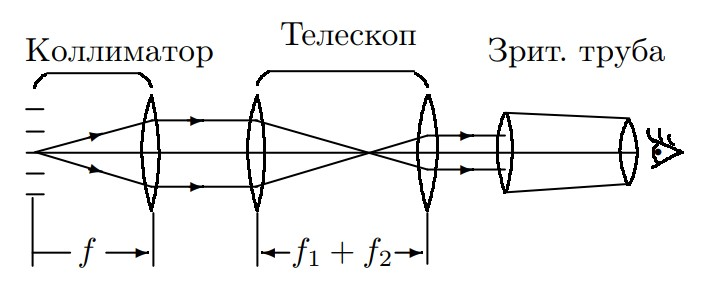
\includegraphics[scale=0.8]{lab_pic3.jpg}
		\caption{Определение увеличения телескопа Кеплера}
  \end{figure}
\subsection{Труба Галилея}
\begin{enumerate}
    \item Не трогая коллиматора и объектива, вместо собирающей окулярной линзы телескопа поставим рассеивающую ($f_{2} = -8 \pm 0,5$ см) на расстоянии от объектива, равном разности фокусов объектива и окуляра. Далее всё выполняется так же, как и в предыдущем пункте, теперь $h_2 = 32 \pm 0,5$
    \item Рассчитаем увеличение телескопа Галилея разными способами.
    \begin{equation}
    N_{\text{Т}} = -\frac{f_{1}}{f_{2}} = 3,5 \pm 0,2
\end{equation}
\begin{equation}
        N_{\text{Т}} = \frac{h_{3}}{h_{1}} = 3,7 \pm 0,2
\end{equation}
\item Результаты разных способов вновь сошлись в пределах погрешности.
\end{enumerate}
\subsection{Модель микроскопа}
\begin{enumerate}
    \item Для создания модели микроскопа с увеличением $N_{\text{М}} = 5$ отберём самые короткофокусные собирающие линзы из набора: $f_{1} = 8 \pm 0,5$ см, $f_2 = 10 \pm 0,5$ см. Рассчитаем необходимые оптический интервал $\Delta$ и длину тубуса $l_{12}$ по формулам ($L = 25$ см - расстояние наилучшего зрения нормального глаза)
        \begin{equation}
        \Delta = \frac{N_{\text{М}}f_{1}f_{2}}{L} = 16,0 \pm 1,3 \text{ см}
    \end{equation}
    \begin{equation}
        l_{12} = \Delta + f_{1} + f_{2} = 34,0 \pm 1,5 \text{ см}
    \end{equation}
    \item Расположим объектив и окуляр на соответствующем расстоянии $l_{12}$ друг от друга. Сфокусируем модель микроскопа на сетку осветителя (глядя невооруженным глазом в окуляр микроскопа, перемещаем осветитель вдоль оптической скамьи до тех пор, пока в окуляре микроскопа не появится
отчётливое увеличенное изображение сетки). Пункту соответствует \textbf{рисунок 4}.
\item Расположим за окуляром модели микроскопа зрительную трубу, настроенную на бесконечность. Слегка перемещая осветитель, получим в поле зрения
трубы изображение миллиметровой шкалы осветителя. Наденем на объектив микроскопа
диафрагму диаметром 1 см и
уменьшим яркость осветителя.
\item Для экспериментального определения увеличения микроскопа измерим величину изображения $ h_{2} = 33 \зь 0,5$ миллиметрового деления предметной шкалы в делениях окулярной шкалы зрительной трубы. Используя результат аналогичных измерений с коллиматорной линзой, фокус
$f = 18,7 \pm 0,5$ см которой известен, рассчитаем увеличение микроскопа по формуле
\begin{equation}
    N_{\text{М}} = \frac{h_{2} L}{h_{1} f} = 4,9 \pm 0,3
\end{equation}
Результат сошёлся с теоретическим значением, равным 5.
 \begin{figure}[h]
 \centering
 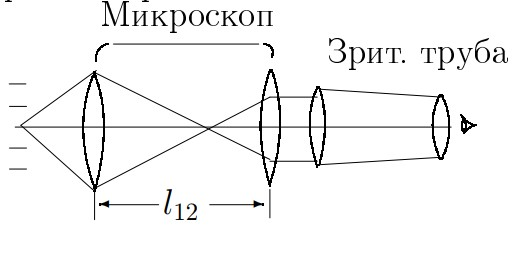
\includegraphics[scale=0.8]{lab_pic4.jpg}
		\caption{Модель микроскопа}
  \end{figure}
    
\newpage
\end{enumerate}
\section{Вывод}
В данной работе было проведено центрирование линз, были определены фокусные расстояния линз, а также смоделированы телескопы Кеплера и Галилея, а также микроскоп. Помимо этого, были рассчитаны увеличения моделей данных приборов (несколькими способами; значения, полученные различными способами оказались равны в пределах погрешности).

\end{document}
